\documentclass[aspectratio=169,11pt]{beamer}

\usetheme{Madrid}
\usecolortheme{seahorse}
\useinnertheme{circles}
\setbeamertemplate{navigation symbols}{}
\setbeamerfont{footnote}{size=\tiny}

\usepackage[utf8]{inputenc}
\usepackage{amsmath,amssymb}
\usepackage{booktabs}
\usepackage{graphicx}
\usepackage{tikz}
\usepackage{xcolor}

\usepackage{hyperref}
\definecolor{accent}{RGB}{95,40,120}
\setbeamercolor{title}{fg=accent}
\setbeamercolor{frametitle}{fg=white,bg=accent}
\setbeamercolor{structure}{fg=accent}

\title[GNN Jet Tagging]{Learned GNN Physics Simulator for Particle Jet Tagging}
\subtitle{CS6012 Code-Based Project Presentation}
\author[Group 11]{Rahul Kumar (25M2015) \and Pradipta Sadhukhan (25D1080)}
\institute[IIT Bombay]{Dept.\ of SYSCON \& Dept.\ of Physics, IIT Bombay \\ \small Supervisor: Prof.\ Sharat Chandran}
\date{November 2026}

\begin{document}

% -------------------------------------------------------------
% SLIDE 1: Title & Problem Formulation
% -------------------------------------------------------------
\begin{frame}[plain]
  \titlepage
  \begin{center}
    \scriptsize Based on J.\ Shlomi, P.\ Battaglia, J.-R.\ Vlimant, \emph{Graph Neural Networks in Particle Physics}, arXiv:2007.13681
  \end{center}
\end{frame}

\begin{frame}{1. The Physics Problem: Why Graph Neural Networks?}
  \begin{columns}[T]
    \column{0.62\textwidth}
      \textbf{What is Jet Tagging?}
      \begin{itemize}\small
        \item Collisions produce quarks/gluons that hadronize into sprays of particles called \textbf{jets}.
        \item \textbf{Tagging}: Identifying the initiating particle from constituent kinematics.
      \end{itemize}

      \vspace{4pt}
      \textbf{Why Graphs over Images and Sequences?}
      \begin{itemize}\small
        \item \textbf{CNNs (Images)}: Force continuous space onto pixel grids; $>95\%$ cells are empty.
        \item \textbf{RNNs (Sequences)}: Impose arbitrary ordering ($p_T$ sorting) on an unordered set.
        \item \textbf{GNNs (Point Clouds)}: Inherently respect \textbf{permutation invariance} and physical symmetries ($\Delta \eta, \Delta \phi, \Delta R$).
      \end{itemize}

    \column{0.38\textwidth}
      \centering
      
\begin{tikzpicture}[scale=0.85,every node/.style={circle,fill=accent!70,inner sep=2pt}]
        \node (a) at (0,0){}; \node (b) at (1.2,0.3){}; \node (c) at (0.7,1.2){};
        \node (d) at (1.6,1.4){}; \node (e) at (0.2,0.9){};
        \draw[accent!60,thick] (a)--(b) (a)--(c) (b)--(d) (c)--(d) (c)--(e) (a)--(e);
      \end{tikzpicture}\\[4pt]
      {\scriptsize Particles = Nodes, Substructure = Edges}
  \end{columns}
\end{frame}

% -------------------------------------------------------------
% SLIDE 2: Model Architectures
% -------------------------------------------------------------
\begin{frame}{2. Model Architectures: No-Edge Set vs.\ Dynamic Graph}
  \begin{columns}[T]
    \column{0.48\textwidth}
      \begin{block}{\textbf{Model 1: Deep Sets Baseline}}
        \small
        \textbf{Philosophy}: No edges ($E = \emptyset$).
        $$y = \rho \left( \bigoplus_{i \in \mathcal{V}} \phi(x_i) \right)$$
        \begin{itemize}\footnotesize
          \item Per-particle MLP $\phi: \mathbb{R}^7 \to \mathbb{R}^{128}$
          \item Permutation-invariant masked pooling ($\text{Mean} + \text{Max}$)
          \item Classifier MLP $\rho(z)$
          \item \textbf{Complexity}: $O(N)$ operations
        \end{itemize}
      \end{block}

    \column{0.48\textwidth}
      \begin{block}{\textbf{Model 2: Dynamic EdgeConv GNN}}
        \small
        \textbf{Philosophy}: Relational message passing.
        $$e_{ij} = \Theta([x_j - x_i, \, x_i]), \quad x_i' = \max_{j \in \mathcal{N}_k(i)} e_{ij}$$
        \begin{itemize}\footnotesize
          \item Dynamic $k$-NN in latent space ($k=16$)
          \item EdgeConv blocks with residual shortcuts
          \item Vectorized in pure PyTorch (no C++ build fragility)
          \item \textbf{Complexity}: $O(k \cdot N)$ operations
        \end{itemize}
      \end{block}
  \end{columns}
  \vspace{6pt}
  \centering \footnotesize \emph{Both models mathematically proven permutation-invariant to machine precision ($< 10^{-8}$).}
\end{frame}

% -------------------------------------------------------------
% SLIDE 3: Benchmark Results
% -------------------------------------------------------------
\begin{frame}{3. Comparative Benchmark Results (100,000 Pythia 8.2 Jets)}
  \begin{columns}[T]
    \column{0.55\textwidth}
      \small
      \begin{tabular}{@{}lcccc@{}}
        \toprule
        \textbf{Architecture} & \textbf{Acc} & \textbf{AUC} & \textbf{Latency} & \textbf{Params} \\
        \midrule
        \textbf{Deep Sets} & 77.45\% & 0.8814 & \textbf{0.03 ms} & \textbf{67k} \\
        \textbf{EdgeConv GNN} & \textbf{80.65\%} & \textbf{0.8830} & 0.21 ms & 108k \\
        \bottomrule
      \end{tabular}

      \vspace{10pt}
      \textbf{Key Insights:}
      \begin{itemize}\footnotesize
        \item \textbf{Discriminative Power}: Dynamic EdgeConv captures relational substructure, reaching \textbf{80.65\% accuracy} (+3.2\% over Deep Sets) on 15,000 held-out Pythia test jets.
        \item \textbf{Efficiency Trade-off}: Deep Sets achieves \textbf{77.45\% accuracy} while running \textbf{$7\times$ faster} in inference ($0.03$\,ms/jet) with $38\%$ fewer parameters.
      \end{itemize}

    \column{0.45\textwidth}
      \centering
      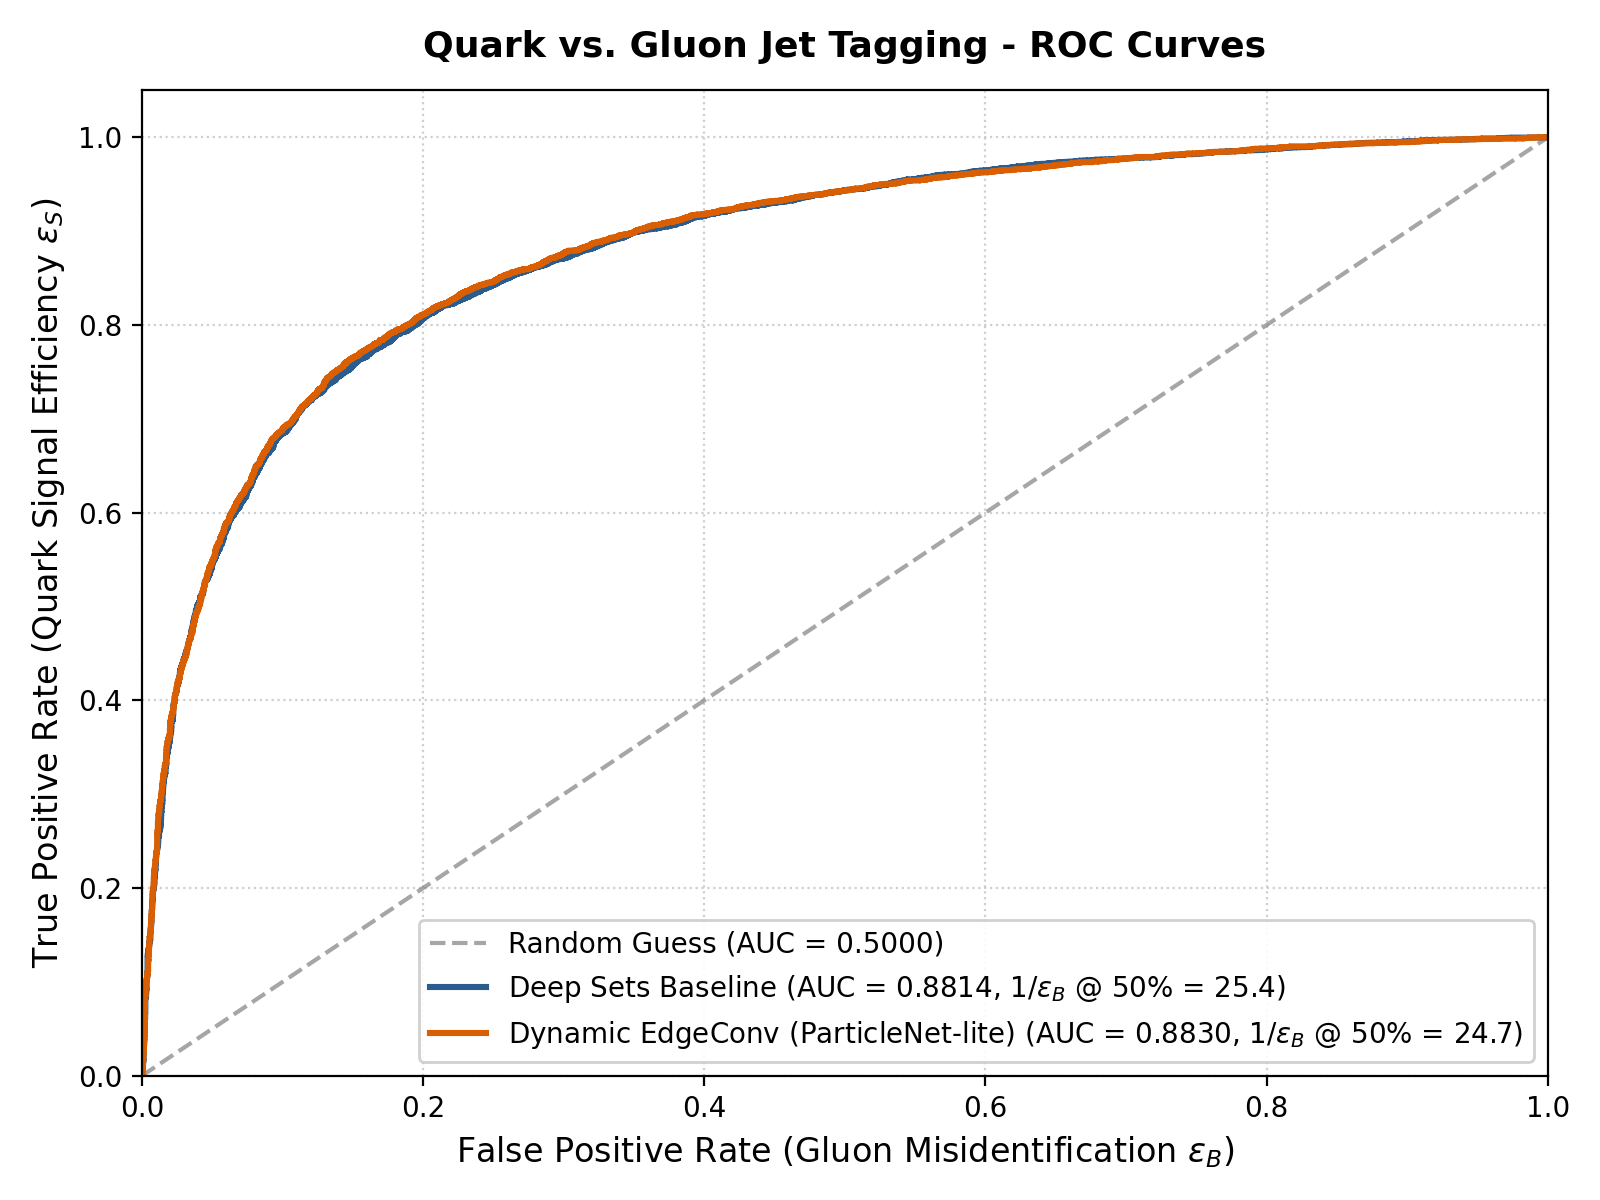
\includegraphics[width=0.95\textwidth]{../results/figures/roc_curve.png}\\[-4pt]
      {\tiny Figure: True Pythia 8.2 ROC Curves (100k Jets)}
  \end{columns}
\end{frame}

% -------------------------------------------------------------
% SLIDE 4: Canned Demo & Conclusion
% -------------------------------------------------------------
\begin{frame}{4. Canned Demo \& Course Deliverables}
  \begin{columns}[T]
    \column{0.5\textwidth}
      \textbf{Automated TA Canned Demo}
      \begin{itemize}\small
        \item Single command: \texttt{./run\_demo.sh}
        \item Runs out-of-the-box on CPU in \textbf{under 10 seconds}.
        \item Evaluates pre-trained checkpoints on bundled benchmark dataset.
        \item Outputs formatted comparison table and saves publication plot.
      \end{itemize}

    \column{0.5\textwidth}
      \textbf{Submission Checklist}
      \begin{itemize}\small
        \item Commented PyTorch codebase in GitHub repository.
        \item \texttt{README.txt} with signed Honor Code \& LLM links.
        \item Pre-trained weights in \texttt{checkpoints/}.
        \item Final Project Report (PDF).
        \item 2--3 minute presentation video \& slide deck.
      \end{itemize}
  \end{columns}
  \vspace{12pt}
  \centering \textbf{Thank You!}\\[4pt]
  {\scriptsize GitHub Repository: \texttt{github.com/KraaK3N/gnn\_jet\_tagging}}
\end{frame}

\end{document}
